\chapter{Theoretische Grundlagen}


\section{Sensoren}

    \subsection{Magnetometer}

    Bei Magnetometern handelt es sich um Sensoren, die das Magnetfeld im Umfeld des Sensors messen können.
    Diese können sowohl in der Luft, als auch auf dem Boden eingesetzt werden.
    Meistens werden für diese Messungen Hall Sensoren oder Induktivitäts-Sensoren verwendet.
    Die Sensoren sind in der Lage, das Magnetfeld in drei Dimensionen zu messen und darzustellen.

    Die Messung des Magnetfeldes erfolgt dabei in der Regel über einen Halbleiter, der durch das Magnetfeld beeinflusst wird.
    und einer Elektronik, die das Signal aufbereitet und ausgibt.
    Magnetometer können jedoch nur die Richtung des Magnetfeldes messen, jedoch nicht die Stärke des Magnetfeldes.
    Magnetometer werden verwendet um die Ausrichtung von Geräten in bestimmten Koordinatensystemen zu bestimmen.
    Sie können für diese Ausrichtungsbestimmung auch in der Luft verwendet werden. 

    \subsection{Kamera} \label{kamera:section}

        \subsubsection{Bild Kamera} \label{bild_kamera:subsubsection}

        \subsubsection{Infrarot Kamera} \label{infrarot_kamera:subsubsection}

    \subsection{Abstandssensoren} \label{abstandssensoren:subsection}

\section{ROS} \label{ros:section}
\ac{ROS} ist eine Open-Source-Plattform, die speziell für die Entwicklung von Robotersoftware entwickelt wurde. Es bietet eine Reihe von Bibliotheken, Tools und Frameworks, die es Entwicklern ermöglichen, komplexe Robotikanwendungen zu erstellen und zu betreiben. \ac{ROS} wurde von Willow Garage entwickelt und ist heute ein weit verbreitetes Framework in der Robotik-Community.

\ac{ROS} besteht aus verschiedenen Modulen, die es ermöglichen, Roboterhard-  und software zu abstrahieren und zu standardisieren. Die Plattform bietet eine Vielzahl von Werkzeugen für die Entwicklung von Robotik-Software, einschließlich Visualisierungstools, Datenverarbeitungs- und Analysetools sowie eine umfassende Dokumentation.

\ac{ROS} ist so konzipiert, dass es auf einer Vielzahl von Betriebssystemen und Hardwarearchitekturen laufen kann und bietet Unterstützung für eine breite Palette von Robotern und Sensoren. Es ist auch bekannt für seine Fähigkeit zur Zusammenarbeit zwischen verschiedenen Robotern, die miteinander kommunizieren und Aufgaben gemeinsam erledigen können.

Dank seiner leistungsstarken Funktionen und Flexibilität ist \ac{ROS} zu einem der wichtigsten Frameworks für die Robotik-Entwicklung geworden und wird in vielen Anwendungen eingesetzt, von industriellen Robotern bis hin zu autonomen Fahrzeugen.

    \subsection{Nodes} \label{nodes:subsection}
    In \ac{ROS} werden Funktionen und Prozesse durch sogenannte Nodes realisiert. Eine Node ist eine ausführbare Einheit, die in einem \ac{ROS}-System arbeitet und über eine eindeutige Identifikation verfügt. Jede Node hat eine spezifische Aufgabe, wie beispielsweise das Sammeln von Sensordaten, die Ausführung einer spezifischen Berechnung oder das Steuern eines Aktors.

    Nodes können miteinander kommunizieren, indem sie Nachrichten senden und empfangen. Nachrichten sind definierte Datenstrukturen, die Informationen zwischen Nodes transportieren. Nodes können auch Services anbieten oder anfordern, um eine bestimmte Aktion auszuführen.

    Eine wichtige Funktion von Nodes ist ihre Fähigkeit zur Verteilung. In \ac{ROS} können Nodes auf verschiedenen Hosts oder in verschiedenen Prozessen ausgeführt werden. Dadurch können komplexe \ac{ROS}-Systeme erstellt werden, die aus vielen miteinander verbundenen Nodes bestehen.

    Nodes können auch in einer \ac{ROS}-Graphenstruktur organisiert werden. Diese Struktur zeigt die Abhängigkeiten zwischen Nodes und die Art der Kommunikation zwischen ihnen an. Die \ac{ROS}-Graphenstruktur kann mit Werkzeugen wie rqt\_graph visualisiert werden, um eine bessere Übersicht über das System zu erhalten.

    Die Verwendung von Nodes in \ac{ROS} ermöglicht eine hohe Flexibilität und Modularität bei der Entwicklung von Robotik-Anwendungen. Entwickler können einzelne Nodes erstellen, testen und optimieren, bevor sie sie in einem größeren System einsetzen. Darüber hinaus können Nodes wiederverwendet werden, um ähnliche Funktionen in verschiedenen Anwendungen auszuführen.

    Insgesamt sind Nodes eine zentrale Komponente von \ac{ROS} und ermöglichen es Entwicklern, komplexe Roboteranwendungen mit einer hohen Flexibilität und Modularität zu erstellen.

    \subsection{Topics} \label{topics:subsection}

    \subsection{Publish and Subscripe Pattern} \label{publish_and_subscripe_pattern:subsection}

    \subsection{Objekterkennung} \label{objekterkennung:subsection}

    \subsection{QR-Codes} \label{qr-codes:subsection}

\section{Drohne/Multicopter} \label{drohne:section}
Bei der für das Projekt verwendete Drohne handelt es sich um eine Coex Clover Drohne. Dies ist eine programmierbare Drohne, die besonders für Bildungszwecke eingesetzt wird. Sie ist sowohl für den Einsatz draußen sowie auch in Gebäuden geeignet. \\

\begin{figure}[htpb]
    \centering
    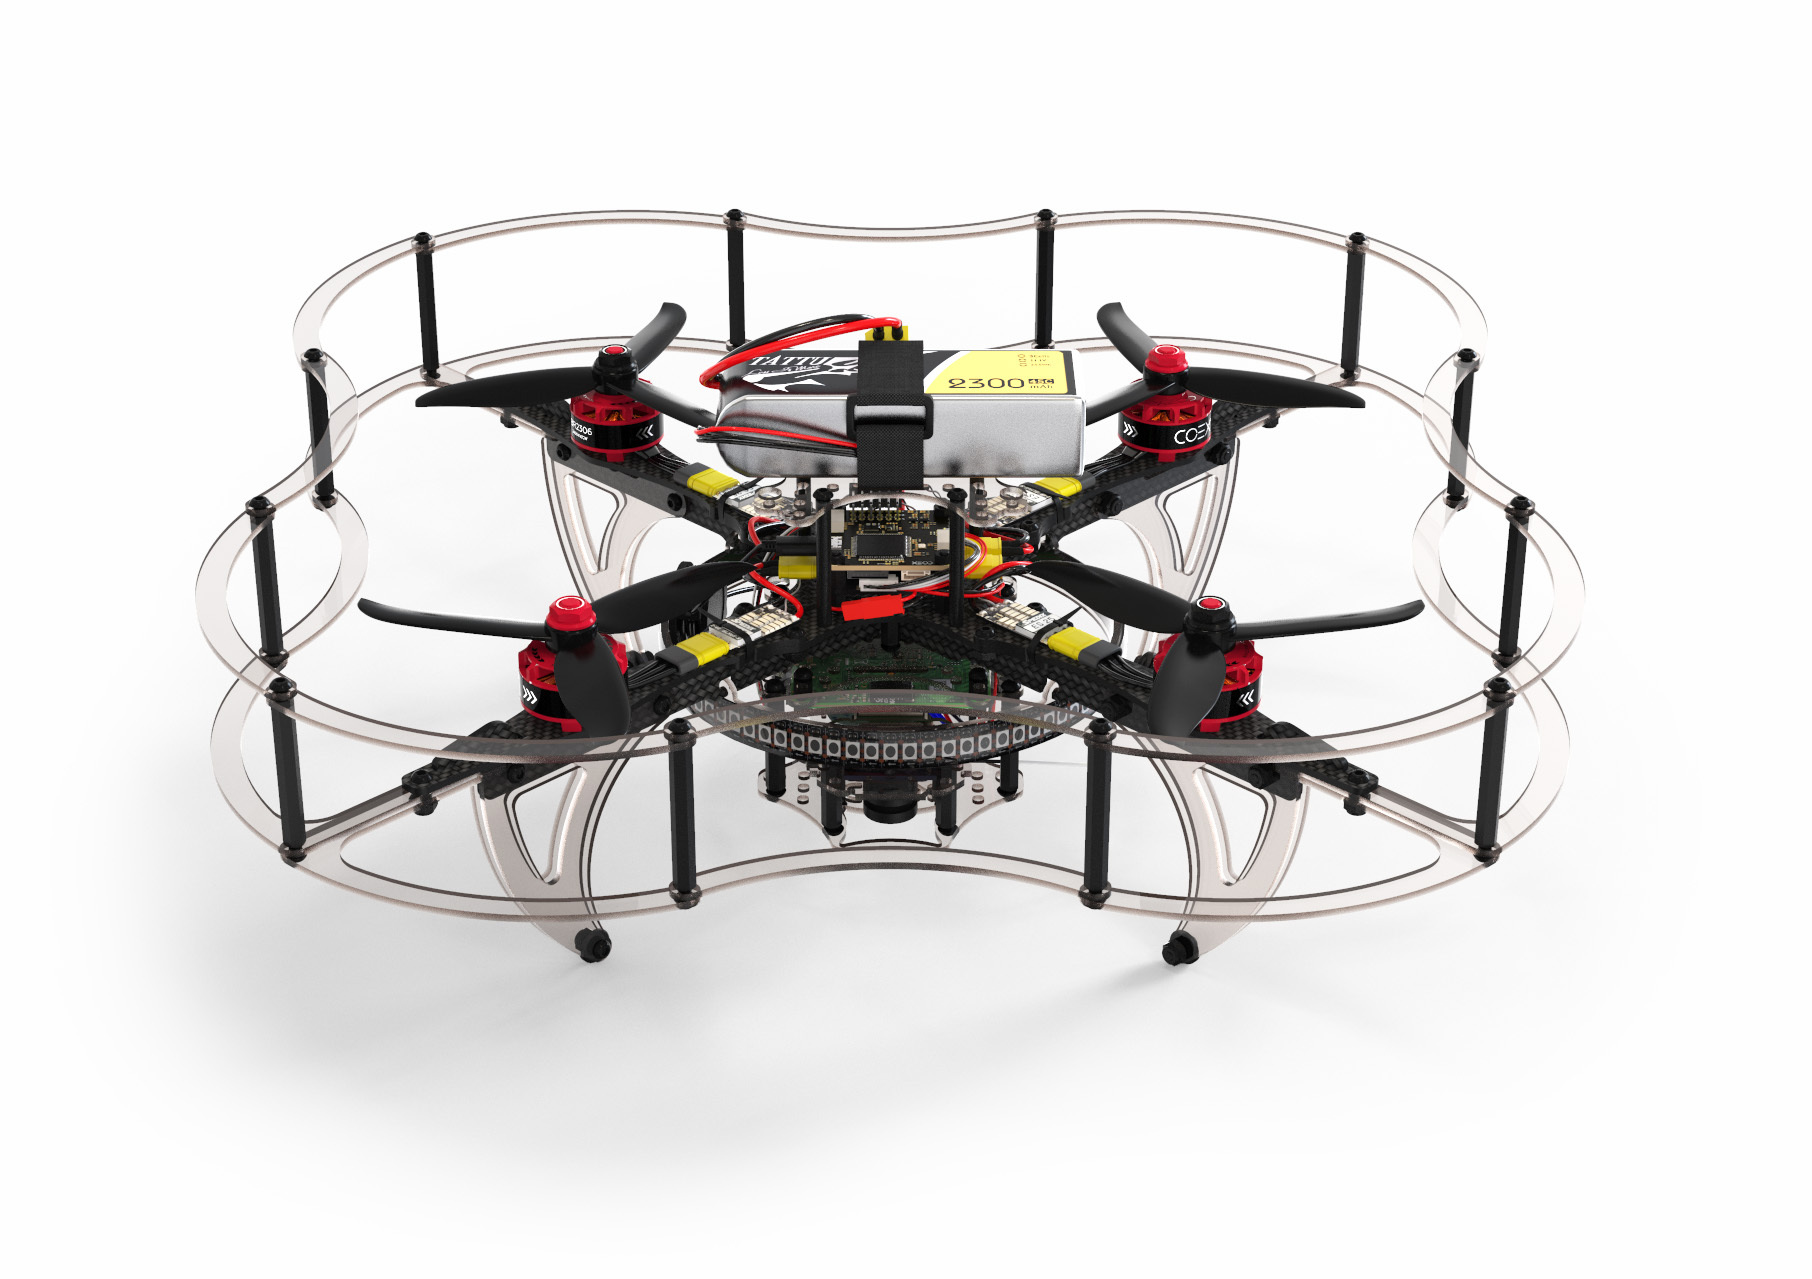
\includegraphics[width=10cm,keepaspectratio,angle=0]{images/coex_clover.jpg}
    \caption[Coex Clover Drohne]{\label{img coex_clover} Coex Clover Drohne \cite{img_coex_clover}}
\end{figure}


Zu Beginn erhält man hierbei einen Bausatz, welcher dann zu einem Quadrokopter zusammengebaut werden kann. Der Vorteil hierbei ist zudem, dass die gesamte Drohne ohne Löten zusammengesetzt werden kann. Zu den einzelnen Bestandteilen der Drohne kommen, noch eine Dokumentation sowie verschiedene Bibliotheken, die es ermöglichen, die Drohne zusammen bauen und fliegen lassen zu können. \\
Die 
Durch die Verwendung verschiedener Open-Source Komponenten lässt sich die Drohne programmieren, wodurch ein vielseitiger Einsatzbereich entsteht.\\





Regenerate response

\begin{figure}[htpb]
    \centering
    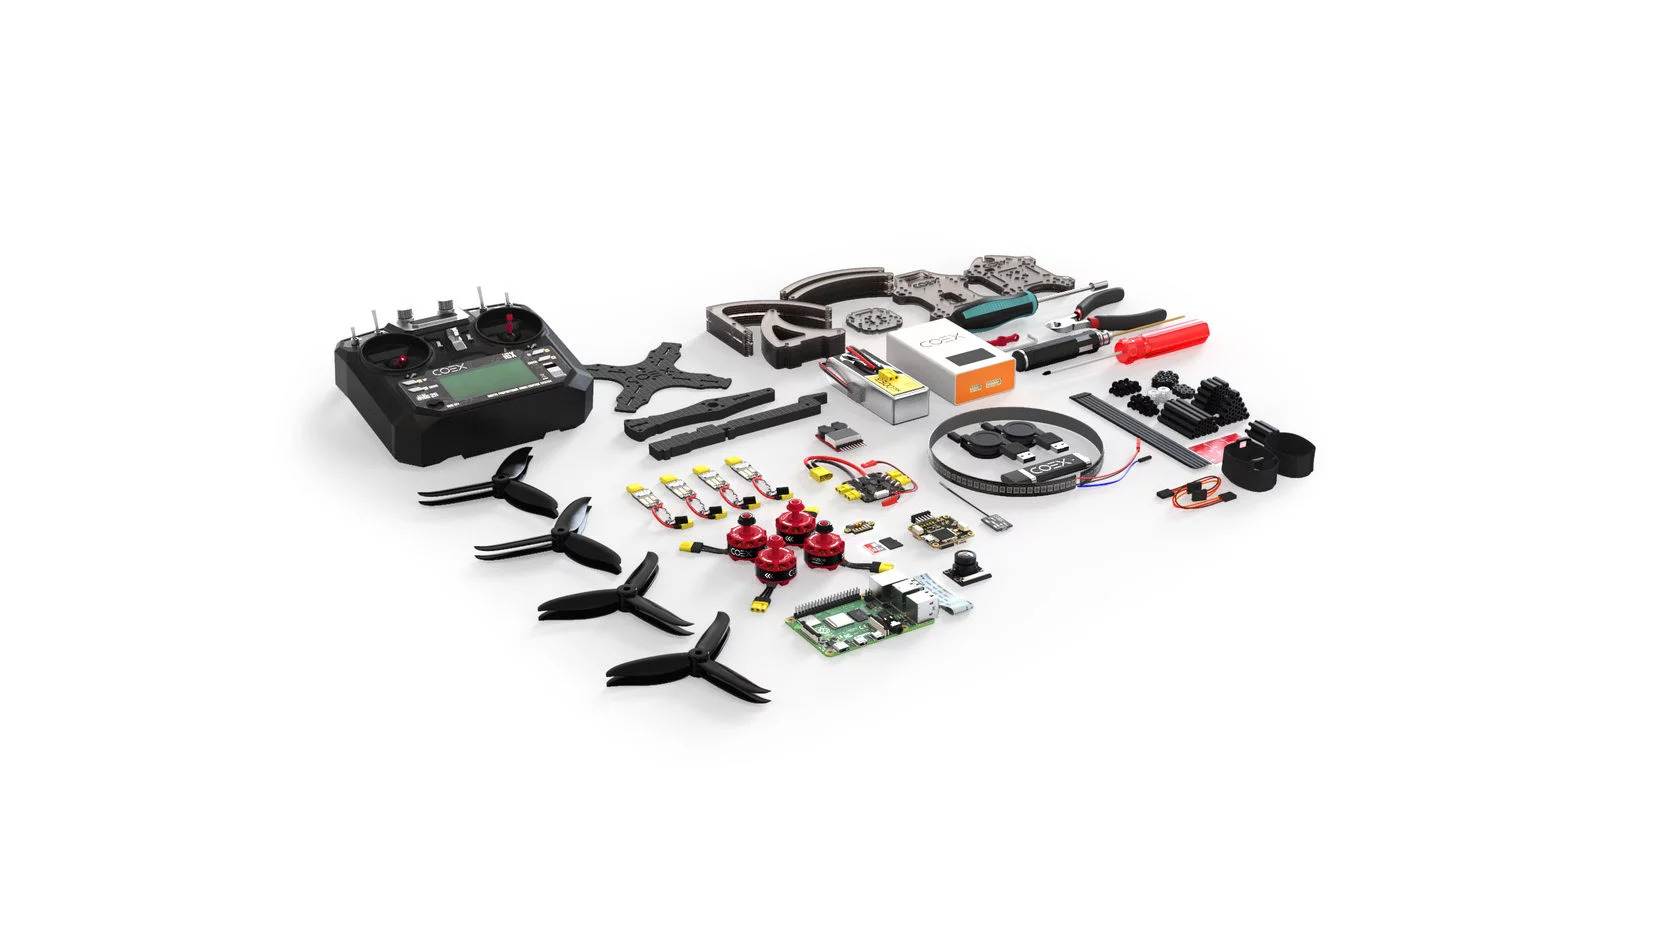
\includegraphics[width=10cm,keepaspectratio,angle=0]{images/coex_clover_kit.jpg}
    \caption[Bausatz Coex Clover Drohne]{\label{img coex_clover_kit} Bausatz Coex Clover Drohne \cite{img_coex_clover_kit}}
\end{figure}

Die Coex Clover Drohne soll laut Herstellerinformationen bis zu 15 Minuten am Stück fliegen können und in dieser Zeit eine Maximalhöhe von 500 Metern bei einer Höchstgeschwindigkeit von bis zu 72 km/h erreichen können \cite[vgl.][]{coex_clover}.\\

Es gibt verschiedene Versionen der Drohne, bei der hier eingesetzten, handelt es sich um die Coex Clover 4.2.
Wichtige Bestandteile dieser sind hierbei:
\begin{center}
    \begin{itemize}
        \item Flight-Controller Coex Pix
        \item Raspberry Pi 4
        \item 
        \item 
        \item 
        \item 
    \end{itemize}
    \label{lst:coex-components}
\end{center}

Zu den Hauptbestandteilen der Drohne zählen zum einen ein Raspberry Pi 4 sowie der Flightcontroller Coex Pix. Diese bilden die Grundlage zur Programmierung und Steuerung der Coes Clover Drohne und ermöglichen es zudem die Drohne über drahtlos per WLAN zu verbinden. \\
Die Drohne ist ein Quadrokopter und besitzt somit vier Motoren, welche einzelnd angesteuert werden können. Sie besitzt zudem eine Vielzahl verschiedener Sensoren, auf welche in Kapitel \ref{sensoren:section} genauer eingegangen wird. Zu diesen zählen unter anderem ein Gyroskop, Magnetometer sowie ein Laseranstandssensor und eine Kamera, die unten an der Drohne angebracht sind.
Zum Schutz befindet sich zudem außen einen Rahmen.



\section{3D-Modelle} \label{3d-modelle:section}

    \subsection{3D-Scanning} \label{3d-scanning:subsection}

\section{Positionsbestimmung} \label{positionsbestimmung:section}

    \subsection{Spatial Mapping} \label{spatial_mapping:subsection}

    \subsection{Inertielle Positionsbestimmung} \label{inertielle_positionsbestimmung:subsection}

\section{Regelsysteme} \label{regelsysteme:section}

    \subsection{PID-Regler} \label{pid_regler:subsection}

\section{Simulationstechnik} \label{simulationstechnik:section}

\section{Problembehebung} \label{problembehebung:section}
